\documentclass[12pt,a4paper]{report}

\usepackage[utf8]{inputenc} % pentru suport diacritice
\usepackage[english]{babel} % setări pentru limba engleza 
\renewcommand\familydefault{\sfdefault} % sans serif

\usepackage[margin=2.54cm]{geometry}	% dimensiuni pagină și margini
\usepackage{graphicx} % support the \includegraphics command and options

% formatting sections and subsections
\usepackage{textcase}
\usepackage{hyphenat}
\usepackage[titletoc, title]{appendix}
\usepackage{titlesec}
\titleformat{\chapter}{\large\bfseries\MakeUppercase}{\thechapter}{2ex}{}[\vspace*{-1.5cm}]
\titleformat*{\section}{\large\bfseries}
\titleformat*{\subsection}{\large\bfseries}
\titleformat*{\subsubsection}{\large\bfseries}

\usepackage{chngcntr}
\counterwithout{figure}{chapter} % no chapter number in figure labels
\counterwithout{table}{chapter} % no chapter number in table labels
\counterwithout{equation}{chapter} % no chapter number in equation labels

\usepackage{booktabs} % for much better looking tables
\usepackage{url} % Useful for inserting web links nicely
\usepackage[bookmarks,
			unicode,
			hidelinks,
			colorlinks = true,
			anchorcolor = blue,
			linkcolor = black,
			urlcolor = blue]{hyperref}

\usepackage{array} % for better arrays (eg matrices) in maths
\usepackage{paralist} % very flexible & customisable lists (eg. enumerate/itemize, etc.)
\usepackage{verbatim} % adds environment for commenting out blocks of text & for better verbatim
\usepackage{subfig} % make it possible to include more than one captioned figure/table in a single float
\usepackage{enumitem}
\setlist{noitemsep}

%%% HEADERS & FOOTERS
\usepackage{fancyhdr}
\pagestyle{empty}
\renewcommand{\headrulewidth}{0pt}
\renewcommand{\footrulewidth}{0pt}
\lhead{}\chead{}\rhead{}
\lfoot{}\cfoot{\thepage}\rfoot{}



\newcommand{\HeaderLineSpace}{-0.25cm}
\newcommand{\UniTextRO}{UNIVERSITATEA POLITEHNICA DIN BUCUREȘTI \\[\HeaderLineSpace] 
FACULTATEA DE AUTOMATICĂ ȘI CALCULATOARE \\[\HeaderLineSpace]
DEPARTAMENTUL DE CALCULATOARE\\}
\newcommand{\DiplomaRO}{PROIECT DE DIPLOMĂ}
\newcommand{\AdvisorRO}{Coordonator științific:}
\newcommand{\BucRO}{BUCUREȘTI}

\newcommand{\UniTextEN}{UNIVERSITY POLITEHNICA OF BUCHAREST \\[\HeaderLineSpace]
FACULTY OF AUTOMATIC CONTROL AND COMPUTERS \\[\HeaderLineSpace]
COMPUTER SCIENCE AND ENGINEERING DEPARTMENT\\}
\newcommand{\DiplomaEN}{DIPLOMA PROJECT}
\newcommand{\AdvisorEN}{Thesis advisor:}
\newcommand{\BucEN}{BUCHAREST}

\newcommand{\frontPage}[6]{
\begin{titlepage}
\begin{center}
{\Large #1}  % header (university, faculty, department)
\vspace{50pt}
\begin{tabular}{p{6cm}p{4cm}}

\includegraphics[scale=0.8]{pics/upb-logo.jpg} &
	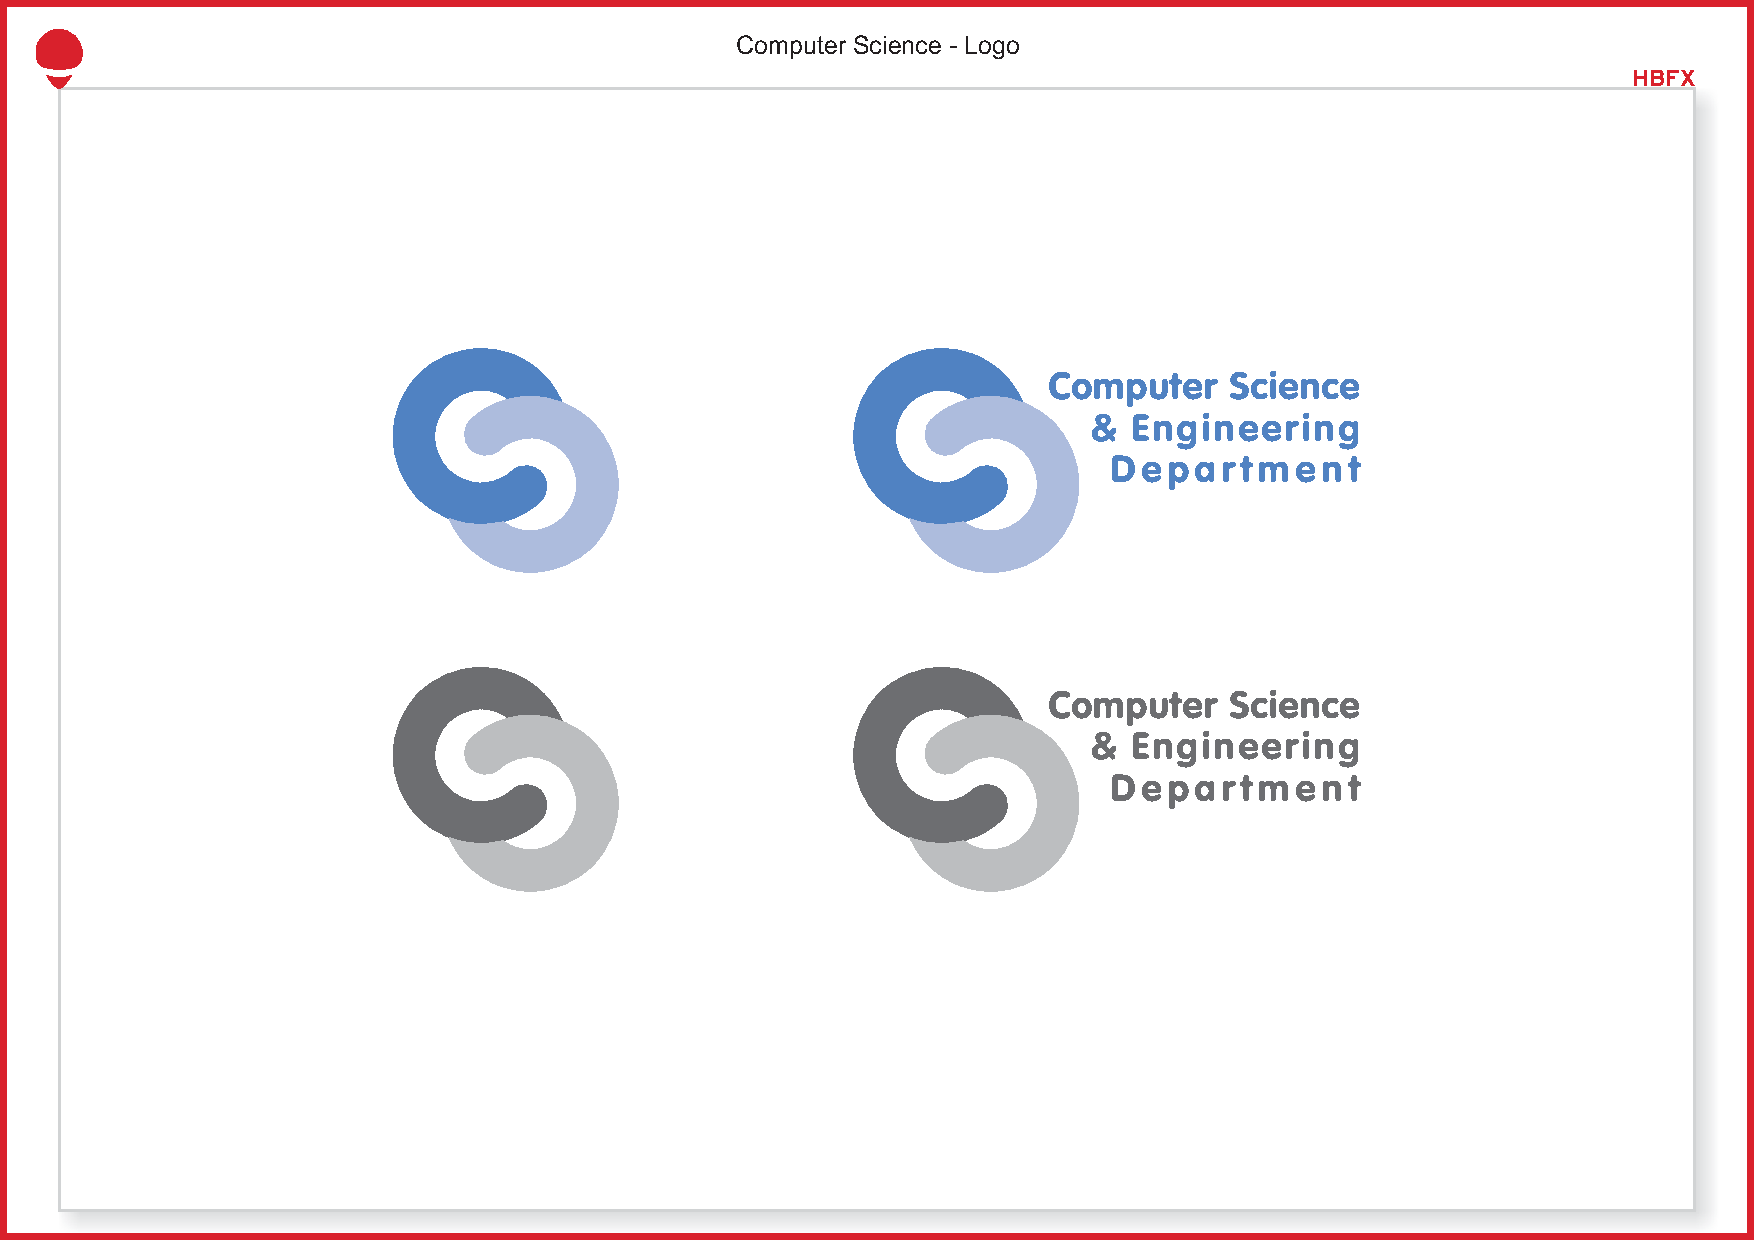
\includegraphics[scale=0.5,trim={14cm 11cm 2cm 5cm},clip=true]{pics/cs-logo.pdf}
\end{tabular}

\vspace{105pt}
{\Huge #2}\\                           % diploma project text
\vspace{40pt}
{\Large #3}\\ \vspace{0pt}  % project title
{\Large #4}\\                          % project subtitle
\vspace{40pt}
{\LARGE \Name}\\                   % student name
\end{center}
\vspace{60pt}
\begin{tabular*}{\textwidth}{@{\extracolsep{\fill}}p{6cm}r}
&{\large\textbf{#5}}\vspace{10pt}\\      % scientific advisor
&{\large \Advisor}                                    % advisor name
\end{tabular*}
\vspace{20pt}
\begin{center}
{\large\textbf{#6}}\\                                % bucharest
\vspace{0pt}
{\normalsize \Year}
\end{center}
\end{titlepage}
}

\newcommand{\frontPageRO}{\frontPage{\UniTextRO}{\DiplomaRO}{\ProjectTitleRO}{\ProjectSubtitleRO}{\AdvisorRO}{\BucRO}}
\newcommand{\frontPageEN}{\frontPage{\UniTextEN}{\DiplomaEN}{\ProjectTitleEN}{\ProjectSubtitleEN}{\AdvisorEN}{\BucEN}}

\linespread{1.15}
\setlength\parindent{0pt}
\setlength\parskip{.28cm}

%% Abstract macro
\newcommand{\AbstractPage}{
\begin{titlepage}
\textbf{\large SINOPSIS}\par
\AbstractRO\par\vfill
\textbf{\large ABSTRACT}\par
\AbstractEN \vfill
\end{titlepage}
}

%% Thank you macro
\newcommand{\ThanksPage}{
\begin{titlepage}
{\noindent \large\textbf{MULȚUMIRI}}\\
\Thanks
\end{titlepage}
}

%% Listing styles
\usepackage{listings}
\usepackage{xcolor}

\colorlet{punct}{red!60!black}
\definecolor{background}{HTML}{EEEEEE}
\definecolor{delim}{RGB}{20,105,176}
\colorlet{numb}{magenta!60!black}

\lstdefinelanguage{json}{
    basicstyle=\scriptsize,
    numbers=left,
    numberstyle=\scriptsize,
    stepnumber=1,
    numbersep=8pt,
    showstringspaces=false,
    breaklines=true,
    frame=lines,
    backgroundcolor=\color{background},
    literate=
     *{0}{{{\color{numb}0}}}{1}
      {1}{{{\color{numb}1}}}{1}
      {2}{{{\color{numb}2}}}{1}
      {3}{{{\color{numb}3}}}{1}
      {4}{{{\color{numb}4}}}{1}
      {5}{{{\color{numb}5}}}{1}
      {6}{{{\color{numb}6}}}{1}
      {7}{{{\color{numb}7}}}{1}
      {8}{{{\color{numb}8}}}{1}
      {9}{{{\color{numb}9}}}{1}
      {:}{{{\color{punct}{:}}}}{1}
      {,}{{{\color{punct}{,}}}}{1}
      {\{}{{{\color{delim}{\{}}}}{1}
      {\}}{{{\color{delim}{\}}}}}{1}
      {[}{{{\color{delim}{[}}}}{1}
      {]}{{{\color{delim}{]}}}}{1},
}



%%%%%%%%%%%%%%%%%%%%%%%%%%%%%%%%%%%%%%%%%%%%%%%%%%   
%%
%%          End of template definitions
%%   
%%%%%%%%%%%%%%%%%%%%%%%%%%%%%%%%%%%%%%%%%%%%%%%%%%


%%% Puteți elimina aceste linii din lucrare, servesc numai pentru template.
\newcommand{\worktype}[1]{[\textit{#1}] }
\newcommand{\dezvoltare}{\worktype{Dezvoltare de produs}}
\newcommand{\cercetare}{\worktype{Cercetare}}
\newcommand{\ambele}{\worktype{Ambele}}
%%%

\addtocontents{toc}{\protect\thispagestyle{empty}}
%%
%%   Campurile de mai jos trebuie modificate de autor. Modificati doar continutul, nu si numele fiecarei definitii
%%
\newcommand{\ProjectTitleRO}{AcadNet.dev}
\newcommand{\ProjectSubtitleRO}{Platformă online pentru rezolvarea problemelor de informatică}
\newcommand{\ProjectTitleEN}{AcadNet.dev}
\newcommand{\ProjectSubtitleEN}{Online platform for solving computer science problems}
\newcommand{\Name}{Dimitrie David}
\newcommand{\Advisor}{Prof. Dr. Ing. Răzvan Victor Rughiniș }
\newcommand{\Year}{2023}

% Setări document
\title{Proiect de diplomă}
\author{\Name}
\date{\Year}

%%
%%   Campurile aferente rezumatului
%%
\newcommand{\AbstractRO}{Această lucrare prezintă \href{https://acadnet.dev}{AcadNet.dev}, o platformă online pentru rezolvarea de probleme de informatică. Platforma oferă un mediu de lucru complet, care permite utilizatorilor să creeze probleme, să le rezolve și să le evalueze automat. Platforma oferă și un mediu de lucru online, care permite utilizatorilor să rezolve problemele direct în browser, fără a fi nevoie să configureze un mediu de dezvoltare local.}

\newcommand{\AbstractEN}{This paper presents \href{https://acadnet.dev}{AcadNet.dev}, an online platform for solving programming problems. The platform offers a complete working environment, which allows users to create problems, solve them and automatically evaluate them. The platform also provides an online working environment, which allows users to solve problems directly in the browser, without the need to configure a local development environment.}

%%
%%   Campurile aferente paginii de multumiri
%%
\newcommand{\Thanks}{(opțional) Aici puteți introduce o secțiunea specială de mulțumiri / acknowledgments. }

\begin{document}

\frontPageRO
\frontPageEN

\begingroup
\linespread{1}
\tableofcontents
\endgroup

\AbstractPage

% Textul licentei incepe de aici 


% INRODUCTION
\chapter{Introduction}\pagestyle{fancy}
\section{Motivation and problem statement}
For the past half year, I was responsible for coordinating the development of problems for the Software Interoperability section of the \href{https://acadnet.ro/}{National Olympiad of Applied Informatics - Acadnet}. This section is different than the regular informatics olympiad, as it focuses more on the engineering side of informatics, rather than the theoretical side. The problems are more practical and require students to be more creative in order to solve them.

The problems are formulated as real life scenarios, where a code is given that should have a certain behavior, but it does not. The students have to find bugs in the code and fix them.

As of right now, there is no accessible methods for students to train for this olympiad. The only way to practice is to solve the problems from the previous years, by downloading their statement and original source. There are no tests to check if the solution is correct. The students have to compile and run the code themselves, and check if the output is correct.

The platform's goal is to create an environment where students can train and prepare for the olympiad in a more efficient way. Moreover, we want to create an online workspace for students, where they can solve problems directly in the browser. This allows us to get more creative with the engineering problems, as we can use more programming languages and configurations, without putting the students through the hassle of setting up a local development environment.

\section{Objectives}
During the last half year, I have been gathering insights on what the students and authors want from a platform like this. I have also been researching the available technologies, and I have been experimenting with different approaches. Based on this, the objectives of this project are defined as follows.

The objective of this project is to create a universal platform for solving engineering tasks. This should include the ability for authors to extend the platform and implement any new language that they want to write a problem in. In addition, the platform should give students the opportunity to solve the tasks directly in the browser, without requiring anything more than an account.
In terms of functionality, the platform should allow authors to create problems, and students to solve them. The platform should also provide a way to automatically evaluate the solutions, and give feedback to the students.

In terms of security, because the solutions will be evaluated by executing user-written code, the platform should be able to run the code in a sandboxed environment, and prevent malicious code from being executed. The platform should also prevent students from cheating, by not allowing them to see the test cases, other users submissions, or the source code of the solutions.

The platform should be easily maintainable, and should be able to scale to a large number of users. It should use containerization to allow for easy deployment and scaling.

\section{Proposed solution and achieved results}
The core of the platform is a web application, which acts as the interface between the users and the platform. The web application is responsible for managing the users, problems, submissions, and for evaluating the submissions. In addition to this, the web application will also be a proxy for online workspaces.

The web application is backed by a SQL database and an S3 file storage. The database is used to store the users, problems, submissions, and other metadata. The file storage is used to store the source code of the problems, and the submissions.

The web application is written in C\# using the .NET Core framework. The database is a PostgreSQL database, and the file storage is an S3 compatible storage, provided by DigitalOcean. The web application is deployed using Helm Charts on a Kubernetes cluster, also provided by DigitalOcean. The checker is written in Python and it is more like an sandbox manager that spawns a new container for each submission, and runs the tests inside the container. Like the checker, the workspace manager is also written in Python, and it is responsible for spawning new workspaces. Workspaces are Docker images based on a Visual Studio Code fork, that allows us to run the code directly in the browser.

The working platform can be found at \href{https://acadnet.dev}{AcadNet.dev} and the source code is open-source and available on Github inside the \href{https://github.com/acadnet-dev}{acadnet-dev} organization.


% PROPOSED SOLUTION
\chapter{System design and architecture}
\section{User journey}
\begin{figure}[h]
	\centering
	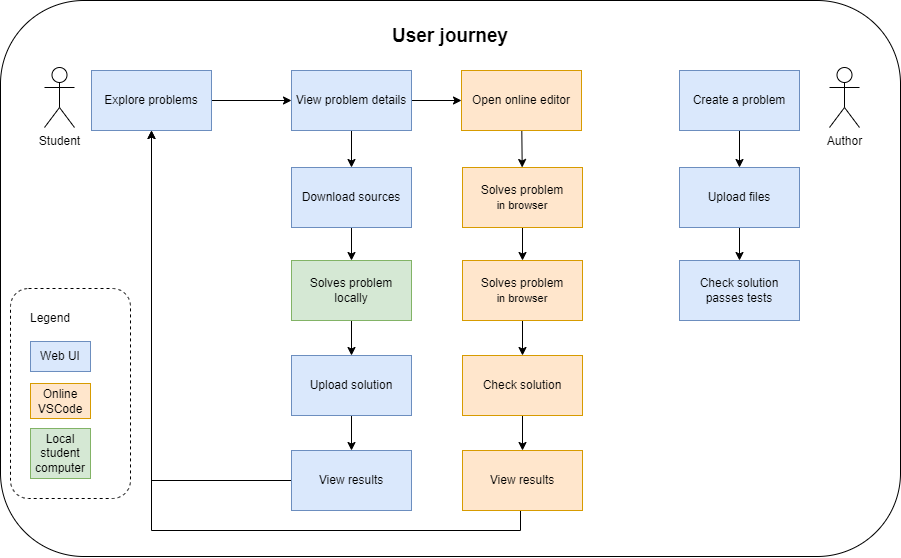
\includegraphics[width=\linewidth]{../photos/user-journey.png}
	\caption{User journey}
	\label{fig:user-journey}
\end{figure}

The platform's main actors are the users that want to learn and practice programming, by solving the problems available. The students can browse the problems, but in order to solve them, they have to create an account. After that, they can choose to solve the problems directly in the browser or they can download the source code and solve them locally. After they solve the problem, they can submit their solution for evaluation. The platform will automatically evaluate the solution, and give feedback to the them.

The other actors are the authors, who are responsible for creating the problems. The authors can create problems, and upload relevant files for the problem. These files include the statement, the source code of the problem, the test cases, and the solution.

\section{Architecture overview}
The architecture is composed of 3 main components: the web application, the checker, and the VSCode workspaces. The web application is the main component, and it is responsible for managing the users, problems, submissions, and for evaluating the submissions. The checker is responsible for evaluating the submissions, and the VSCode workspaces are used to allow users to solve the problems directly in the browser. The block diagram of the architecture can be seen in the figure below.

\begin{figure}[h]
	\centering
	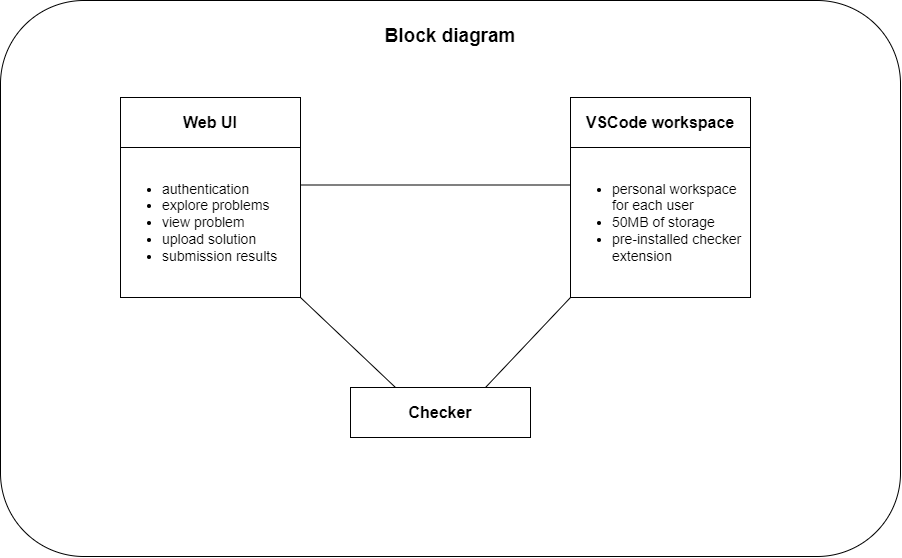
\includegraphics[width=\linewidth]{../photos/block-diagram.png}
	\caption{Software block diagram}
	\label{fig:software-architecture}
\end{figure}

\begin{table}[th]\small\linespread{1}
\caption{Component's responsibilities}
\label{tab:criterii}
\begin{tabular}{l >{\raggedright\arraybackslash}p{10cm} >{\raggedright\arraybackslash}p{0cm}}
\textbf{Component} & \textbf{Responsibilities} \\\hline
\textbf{Web App} & Manage users, problems and submissions; send submissions to the checker and present results; manage VSCode workspaces & \\
\hline
\textbf{Checker} & Test submissions by spawning a new sandbox in the K8s cluster and compare reference outputs with actual outputs & \\
\hline
\textbf{VSCode workspace} & Allow users to solve problems directly in the browser & \\
\hline
\end{tabular}
\end{table}

\newpage
\section{System components and interactions}
The web app is the brain of the platform. It is interacting with all the other components. With regards to the checker, the web app is responsible for receiving the submissions from the user or from the online workspace and to send them to the checker. While the checker is evaluating the submission, the web app constantly polls the checker for the updates and results. When the checker is done, the web app will receive the results and will update the submission with the status. On the other hand, when it comes to the interaction with the online workspaces, the web app is responsible for spawning new workspaces via the workspace manager and it acts as a HTTP and websocket proxy between the user's browser and the workspace.

\begin{figure}[h]
	\centering
	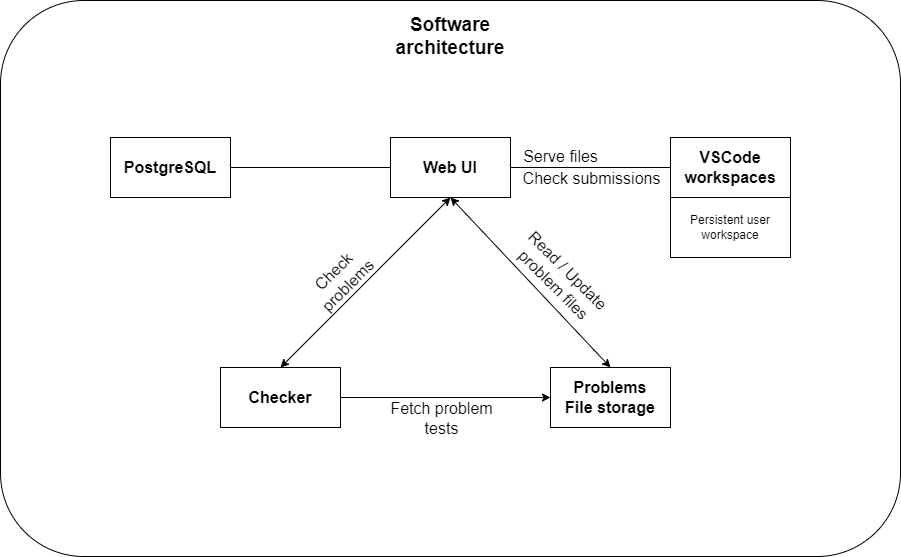
\includegraphics[width=\linewidth]{../photos/software-architecture.png}
	\caption{System components and their interactions}
	\label{fig:system-components}
\end{figure}

\subsection{SQL and file storage}
Other than the 3 main components, the architecture also includes a SQL database and an S3 file storage. The database is used to store the users, problems, submissions, and other metadata. The file storage is used to store the source code of the problems, and the submissions. The interactions between the components can be seen in the figure below. The web application is the only component that interacts with the database. With the file storage, the web application and the checker interact with it. The web application uses it to store the files uploaded by the authors, and the checker uses it to pull the test cases for the problem.


\section{Database design}
The database is designed using an ORM (Object Relational Mapper) called Entity Framework. This allows us to define the database schema using C\# classes, and because we are using a "code first" approach, the database tables and relations will be created automatically, using migrations. The database schema can be seen in the figure below. 

\begin{figure}[h]
	\centering
	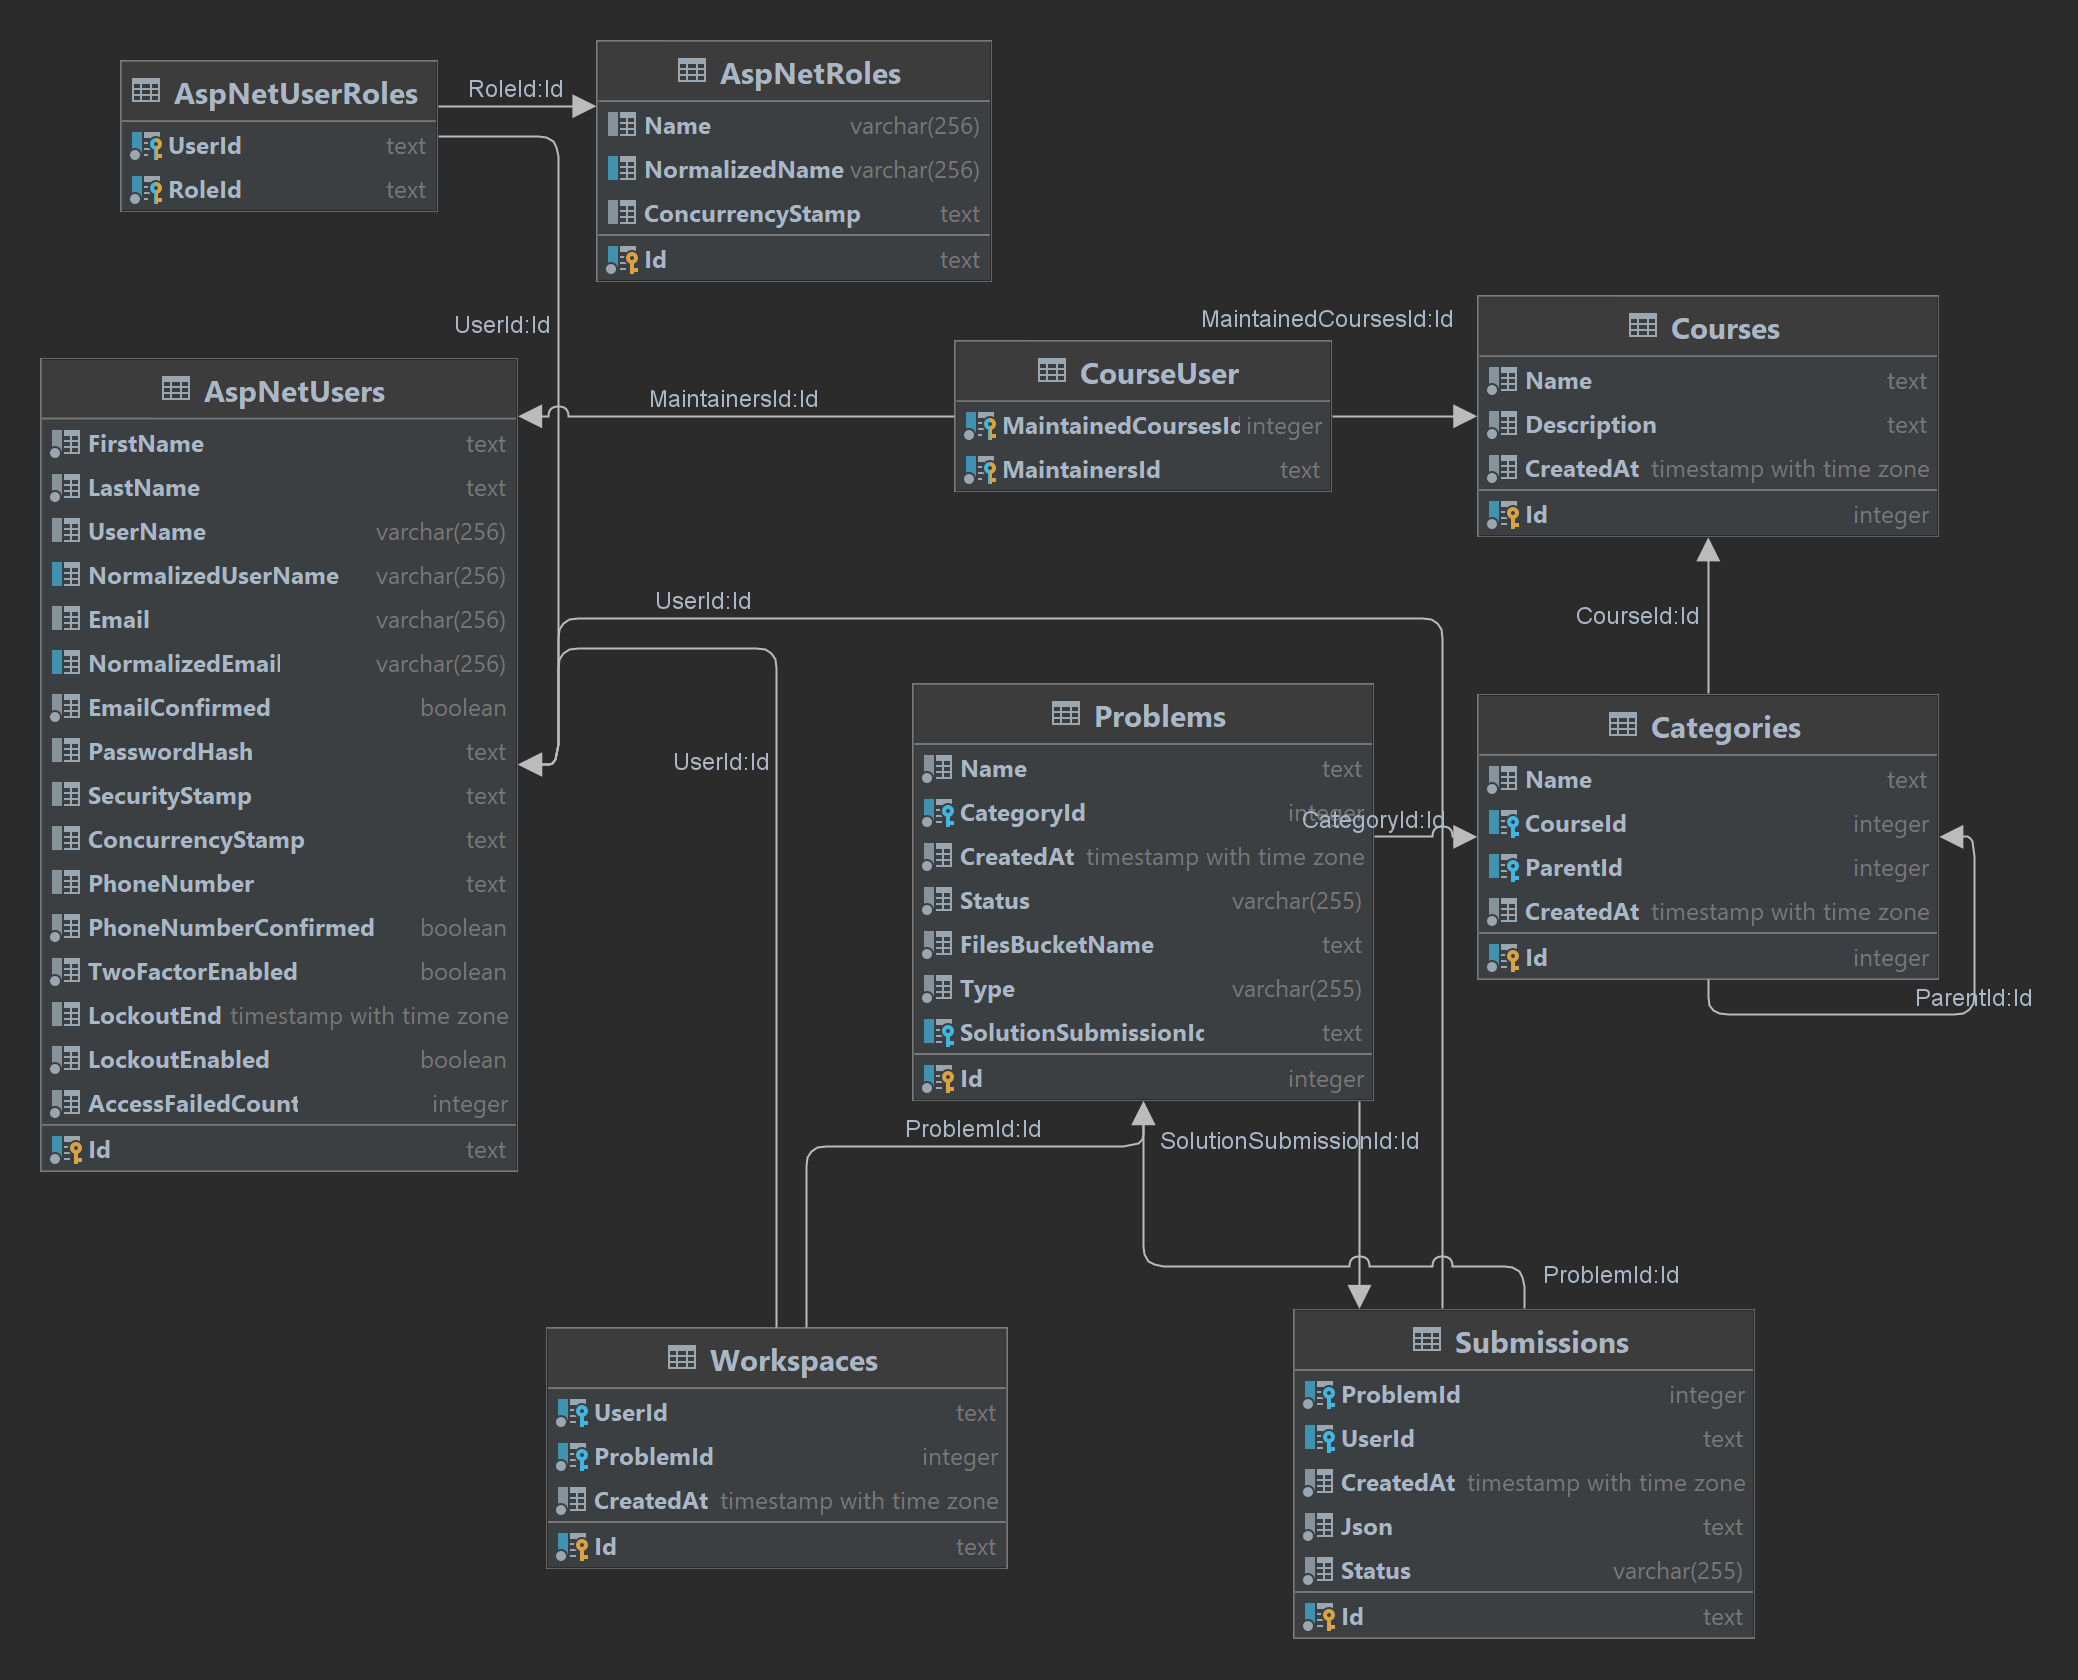
\includegraphics[width=\linewidth]{pics/database-schema.png}
	\caption{Database schema diagram}
	\label{fig:database-schema}
\end{figure}

As we can see in Figure \ref{fig:database-schema}, the database is composed of multiple tables. Some of them are automatically generated by the .NET Identity Framework that handles authentication.

Below is a description of each table and its purpose.

\newpage
\subsection{Users and roles}
\begin{itemize}
	\item \textbf{AspNetUsers} - stores the users that have an account on the platform. The users can be either students or authors.
	\item \textbf{AspNetRoles} - stores the roles available on the platform. Currentyl, there are only 2 roles: student and author.
	\item \textbf{AspNetUserRoles} - because the realtion between users and roles is many to many, this table is used to store what roles each user has.
\end{itemize}

\subsection{Problem hierarchy}
The problems are organized in a tree-like structure. As the root there are the courses that have a name and a description. Each course have multiple categories, and each category can have as children other categories or problems. An example of the hierarchycal structure is shown in Figure \ref{fig:problem-hierarchy}.

\begin{figure}[h]
	\centering
	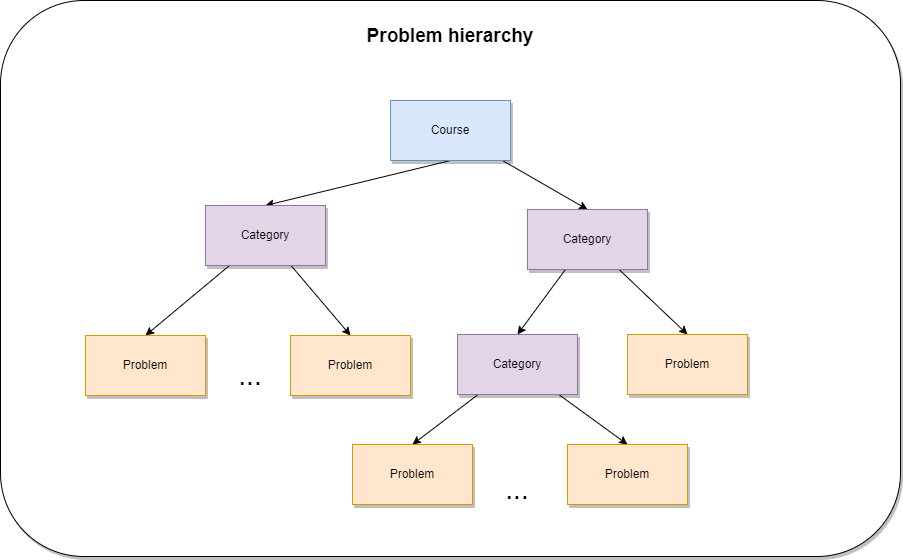
\includegraphics[width=\linewidth]{../photos/problem-hierarchy.png}
	\caption{Problem hierarchy}
	\label{fig:problem-hierarchy}
\end{figure}

\begin{itemize}
	\item \textbf{Courses} - stores the courses available on the platform.
	\item \textbf{CourseUser} - a course can have maintainers. This table stores the relation between the courses and the users that are maintainers.
	\item \textbf{Categories} - stores the categories available on the platform. Each category have a course and may have a parent category.
	\item \textbf{Problems} - stores the problems available on the platform. Each problem have a category. Also, the problem stores the bucket id of the file storage where the problem's files are stored.
\end{itemize}

\subsection{Submissions and workspaces}

\begin{itemize}
	\item \textbf{Submissions} - stores the submissions made by the users. Each submission have a problem and a user.
	\item \textbf{Workspaces} - stores the workspaces available on the platform. Each workspace have a problem and a user.
\end{itemize}

% IMPLEMENTATION DETAILS
\chapter{Implementation details}
All the code for the platform and all its components is available on Github inside the \href{https://github.com/acadnet-dev}{acadnet-dev} organization.

\section{Web application}
The web application is the main component of the platform. It is responsible for managing the users, problems, submissions, and for evaluating the submissions. In addition to this, the web application acts as a proxy for the online workspaces. The web application is written in C\# using the .NET Core framework. It is using the MVC (Model-View-Controller) pattern, and it is using an ORM (Object Relational Mapper) called Entity Framework to interact with the database. The web application is deployed as a Docker image using multi-stage builds. The Docker image is deployed on a Kubernetes cluster using Helm Charts. The web application is composed of multiple components, which are described below.

\subsection{Controllers}
The controllers are the components that handle the HTTP requests. They receive a request from the user, process it by calling different services and interacting with other components so that it returns a response. The platform has multiple controller, each acting in its own domain. The controllers are described below.

\textbf{AuthController}
It handles all the actions related to user authentication and authorization. It is responsible for registering new users, logging in existing users, and managing the user's roles.

Registering users and logging in users is done via external authentication providers. Currently, the platform only supports Google authentication, but it can be easily extended to support other providers. Support for other popular external providers is already implemented in the .NET framework.

\textbf{CoursesController}
It handles all the actions related to courses like creating new courses. This action can be done only by users that have the author role. It also handles creating categories and listing the hierarchycal structure of the courses so that users can browse them.

\textbf{ProblemsController}
This controllers controls all the actions related to problems. It handles creating new problems, showing the problem's statement, and evaluating the submissions. Problems can only be created if the user created the respective course and is a maintainer of the course.

Submitting a solution is done by uploading a file with the solution's source code. The file is sent to the checker. There is also a `GET` endpoint that returns the submission's status. This endpoint is called periodically by the frontend to check if the submission is done.

\textbf{WorkspaceController}
This controller is responsible for managing the online workspaces. It handles creating new workspaces, and sets the environment for the proxy to connect to the workspace. More details about the proxy and how the workspaces are accessed by the user's browser can be found in Section \ref{workspaces-proxy}.

\subsection{UI}
The UI is built using the Razor Pages framework. It is created based on a template from \href{https://themeforest.net/}{Theme Forest}.
In terms of technologies, the UI uses SASS, jQuery, and Bootstrap. The UI is responsive and it works on both desktop and mobile devices.

Some of the interesting elements that the UI has are described below.

\textbf{Problem statement}
The problem author's are required to upload a Markdown file with the problem's statement. The UI is using the \href{https://github.com/xoofx/markdig}{Markdig} library to convert the Markdown file to HTML. The HTML is then rendered in the browser using custom CSS styles for the different elements in Markdown.

\textbf{File upload}
The file upload input is a custom component that is using the \href{https://pqina.nl/filepond/}{FilePond} library. This library is responsible for creating a responsive and dynamic file upload input. It lets authors upload multiple files at once and remove already uploaded files. It also has a drag and drop feature, and it can be easily extended to support other features like file validation, file preview, and image editing. 

\begin{figure}[h]
	\centering
	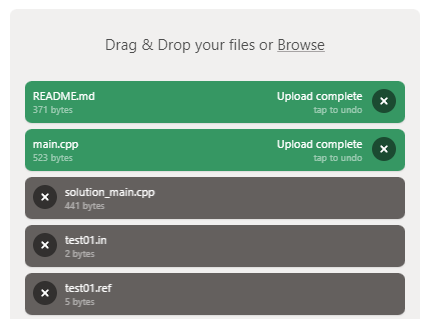
\includegraphics[width=250px]{./pics/file-uploader.png}
	\caption{File upload component}
	\label{fig:file-upload}
\end{figure}

\newpage
\subsection{Services}
The services are the components that handle the business logic of the platform. They are used by the controllers to process the requests. They are responsible for interacting with the database and the file storage. Services are a pair made of an interface describing the available methods, and a class implementing the interface. Services are using a dependency injection mechanism to be injected into the controllers and other services. The functionality of each service is described below.

\textbf{FileService}
This service is responsible for interacting with the file storage. It is used to create buckets\protect\footnotemark{} and upload and download files from the file storage.
\footnotetext{A bucket is a collection of files in an S3 compatible storage}

\textbf{ProblemService}
This service handles all the actions regarding problems. It is implemented using the Factory design pattern, because the problems can be written in different languages and have different methods of evaluation and initialization. Currently, the platform implements only one type of problem with one file source code of C++ and tests that are based on finding differences between the reference output and the actual output. But it can be easily extended to support other types of problems, written in other languages, and with other methods of evaluation like asserting the execution time or the memory usage.

Some of the methods that needs to be implemented for each type of problem are described below.

\begin{itemize}
	\item creating a problem
	\item getting a problem by id
	\item getting a problem's statement and converting it from Markdown to HTML
	\item get the sources of a problem to be downloaded by the user
	\item get the test cases of a problem so that they can be sent to the checker
	\item creating and updating a submission
	\item getting the necessary files to initialize a workspace
\end{itemize}

\textbf{CheckerService}
This service is responsible for interacting with the checker. It is used to create submissions and to get the status of a submission.

\textbf{WorkspaceService}
This service is responsible for interacting with the workspace manager. It is used to create workspaces and to get the url of a workspace for the proxy redirect.

\subsection{Workspaces Proxy} \label{workspaces-proxy}
The workspaces proxy is a component that acts as an intermediate between the user's browser and the workspace. It is responsible for receiving user requests for the workspace and redirecting them to the appropriate workspace container. It also handles the websocket connections between the user's browser and the workspace container.

The proxy is written as a middleware in .NET Core and it is part of the web application. Because of this, it is very easy to check if the user is authenticated and authorized to access the workspace, because the authentication cookies are already in the user's browser and are transmitted with each request. 

\section{SQL database}
The SQL database is a PostgreSQL database. It is deployed as a managed service on DigitalOcean. The database is used to store the users, problems, submissions, and other metadata. The database schema can be seen in Figure \ref{fig:database-schema}. The web application is the only component that interacts with the database. It is controlled using Entity Framework, which is an ORM (Object Relational Mapper) that allows us to define the database schema using C\# classes. The database tables and relations are defined in a "code-first" approach, which means that the tables and relations are created by the ORM by translating the C\# classes and relationship between them to tables and keys.

Each modification to the database schema is handled by migrations. Migrations are C\# classes that describe the changes that need to be made to the database schema. The migrations are created automatically by the ORM, and they are applied automatically when the application starts. This allows for easy modifications on the database schema without having to manually create the tables and relations.

\section{File storage}
The platform needs a distributed storage method for the files uploaded by the authors and the submissions made by the users. An S3 compatible storage is a good solution for this, because it is easy to use and it is scalable. For this project, when developing we are running a local S3 compatible storage using \href{https://min.io/}{MinIO}. For production, we are using a managed S3 compatible storage provided by DigitalOcean called \href{https://www.digitalocean.com/products/spaces/}{Spaces}.

The storage is accessed using Amazon's S3 C\# SDK. The SDK is used to create buckets, upload and download files, and list files in a bucket. The buckets are created automatically by the web application when a new problem is created. The bucket's name is a UUID. The files are uploaded with specific names, defined by the problem type.

\newpage
For example, for the C++ problems, the files are uploaded with the following names.

\begin{itemize}
	\item \textbf{main.cpp} - the source code of the problem
	\item \textbf{soltion\_main.cpp} - the source code of the solution
	\item \textbf{README.md} - the statement
	\item \textbf{test0.in} - the first test case
	\item \textbf{test0.ref} - the first test case's reference output
	\item \textbf{test1.in} - the second test case
	\item \textbf{test1.ref} - the second test case's reference output
	\item \textbf{...}
\end{itemize}

\section{Checker}
The checker is the component of the platform that handles the evaluation of the submissions. It is written in Python and it is exposed as a simple REST API. The checker is deployed as a Docker image on the Kubernetes cluster. The checker is composed of multiple components, which are described below.

\subsection{API}
The API is built using the \href{https://fastapi.tiangolo.com/}{FastAPI} framework. It is a simple REST API that exposes 2 endpoints: one for creating a new submission, and one for getting the status of a submission. The API is responsible for receiving the submission from the web application, and for sending the results back to the web application.

The API endpoints are described below.

\textbf{POST /submission/create}

% TODO: describe the request and response
\begin{description}
	\item[Query parameters]\
		\begin{itemize}
			\item \textbf{type} - the type of the problem
			\item \textbf{bucket} - the bucket id where the problem's files are stored
		\end{itemize}
	\item[Request body]\
		\begin{itemize}
			\item \textbf{file} - the file with the source code of the submission as a multipart form data
		\end{itemize}
	\item[Response body]\
		\begin{itemize}
			\item \textbf{submission\_id} - the id of the newly created submission
		\end{itemize}
\end{description}

\newpage
\textbf{GET /submission/status}
\begin{description}
	\item[Query parameters]\
		\begin{itemize}
			\item \textbf{submission\_id} - the id of the submission
		\end{itemize}
	\item[Response body]\
		\begin{itemize}
			\item \textbf{status} - the status of the submission
		\end{itemize}
\end{description}

An example of a submission status for a C++ problem can be seen in the appendix \ref{anexa:cod:json-submission}. Important things to be noted are the presence of the compilation status, the expected and actual results for each test case and all the logs from the sandbox.

\subsection{Sandbox adapter}
The purpose of the sandbox adapter is to communicate with the Kubernetes cluster and with the Sandbox itself, for things like creating the sandbox, uploading files to the sandbox, running commands inside the sandbox or purging the sandbox after the submission is evaluated.

When creating a submission, the actual thing that happens is that a new sandbox is launched so that the code can be executed inside it. The sandbox is a Docker container that is launched on the Kubernetes cluster. The sandbox is controlled with the \href{https://github.com/kubernetes-client/python}{Python Kubernetes client}. The launched sandbox depends on the type of problem that is being evaluated. This way we can have different types of problems, written in different languages, and with different methods of evaluation and the sandbox will have all the resources needed to evaluate the submission.

The interactions between the checker and other components can be seen in Figure \ref{fig:checker-interactions}.
\begin{figure}[h]
	\centering
	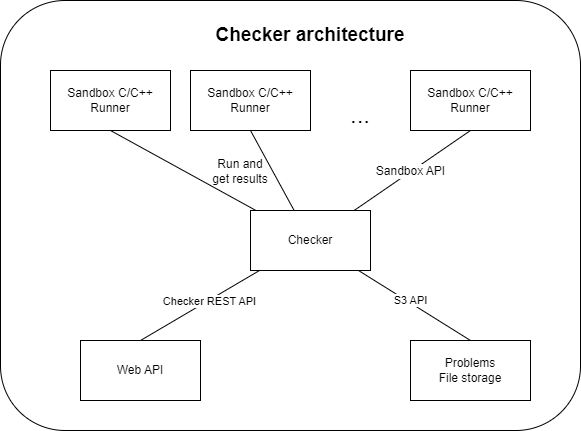
\includegraphics[width=300px]{../photos/checker-architecture.png}
	\caption{Checker interactions}
	\label{fig:checker-interactions}
\end{figure} 


\subsection{File manager}
All the files that come to the checker, being them received from the web application or downloaded from the file storage, are stored in a temporary directory. The file manager is responsible for managing the files in this directory. It is responsible for creating the directory, uploading files to the directory, and deleting the directory when the submission is evaluated.

\subsection{Submission factory}
The submission factory is responsible for creating the submission object, based on the problem type. The implementation of the submission object is different for each type of problem. It needs to know stuff like what commands to run to build the code, how do the tests look, how to run them and how to compare the results. Currently, the platform only supports one type of problem, but it can be easily extended to support other types of problems.

\subsection{Workflow for C++ problems}
\begin{enumerate}
	\item The checker receives a new submission from the web application via the API.
	\item The checker stores the submitted file in a temporary directory.
	\item Based on the problem type, the checker creates a new submission object.
	\item The submission object fetches all the necessary files from the file storage.
	\item The sandbox adapter creates a new sandbox on the Kubernetes cluster.
	\item The sandbox adapter uploads all the necessary files to the sandbox.
	\item The sandbox adapter runs the build command inside the sandbox.
	\item The sandbox adapter iterates through all the test cases and runs them inside the sandbox.
	\item The sandbox adapter compares the actual output with the reference output and stores the results.
	\item The sandbox adapter deletes the sandbox.
\end{enumerate}


\subsection{Global status object}
All the submissions are run in a background thread. The status is a global object that is updated by the sandbox adapter as it progresses through the workflow. When the API receives a request for the status of a submission, it returns the status object.

\section{Sandbox image}

\section{VSCode workspaces manager}
3

\section{VSCode online image}

\section{VSCode checker extension}


% FEATURES AND FUNCTIONALITIES
\chapter{Features and functionalities}
\section{User authentication}
1

\section{Problem creation}
1

\section{Problem browsing}
1

\section{Problem solving}
1

\section{Submission evaluation}
1

\section{Online workspaces}
1



% DEPLOYMENT AND MAINTENANCE
\chapter{Deployment and maintenance}
\section{Infrastructure}
3

\section{Continuous integration}
2

\section{Continuous deployment}
2

\section{Monitoring}
1



% TESTING AND VALIDATION
\chapter{Testing and validation}
Read in template.pdf
\section{Evaluation criteria}
1

\section{Performance}
1

\section{Security}
1

\section{User feedback}
2



% CONCLUSIONS AND FUTURE WORK
\chapter{Conclusions and future work}
\section{Conclusions}
1

\section{Future enhancements}
1

\section{Lessons learned}
1


% BIBLIOGRAPHY
\chapter*{Bibliography}\addcontentsline{toc}{chapter}{Bibliography}  
% * <marios.choudary@gmail.com> 2018-02-28T12:07:48.730Z:
% 
% > BIBLIOGRAFIE
% Am adaugat un paragraf cu cateva detalii despre folosirea citarilor bibliografice in Latex, despre folosirea lui "\cite" si despre posibilitatea folosirii bibliografiei si direct in fisierul Latex.
% 
% ^.

\begin{itemize}
	\item 	NU utilizați referințe la Wikipedia sau alte surse fără autor asumat.
	\item 	Pentru referințe la articole relevante accesibile în web (descrise prin URL) se va nota la bibliografie și data accesării.
	\item 	Mai multe detalii despre citarea referințelor din internet se pot regăsi la:
	\begin{itemize}
		\item	\url{http://www.writinghelp-central.com/apa-citation-internet.html}
		\item	\url{http://www.webliminal.com/search/search-web13.html}
	\end{itemize}
	\item 	Note de subsol se utilizează dacă referiți un link mai puțin semnificativ o singură dată; Dacă nota este citată de mai multe ori, atunci utilizați o referință bibliografică.
	\item 	Dacă o imagine este introdusă în text și nu este realizată de către autorul lucrării, trebuie citată sursa ei (ca notă de subsol sau referință - este de preferat utilizarea unei note de subsol).
	\item 	Referințele se pun direct legate de text (de exemplu ``KVM [1] uses'', ``as stated by Popescu and Ionescu [12]'', etc.). Nu este recomandat să folosiți formulări de tipul ``[1] uses'', ``as stated in [12]'', ``as described in [11]'' etc..
	\item 	Afirmațiile de forma ``are numerous'', ``have grown exponentially'', ``are among the most used'', ``are an important topic'' trebuie să fie acoperite cu citări, date concrete si analize comparative.
	\begin{itemize}
		\item	Mai ales în capitolele de introducere, ``state of the art'', ``related work'' sau ``background'' trebuie să vă argumentați afirmațiile prin citări. Fiți autocritici și gândiți-vă dacă afirmațiile au nevoie de citări, chiar și cele pe care le considerați evidente.
		\item	Cea mai mare parte dintre citări vor fi în capitolele de introducere ``state of the art'', ``related work'' sau ``background''.
	\end{itemize}
	\item 	Toate intrările bibliografice trebuie citate în text. Nu le adăugați pur și simplu la final.
	\item 	Nu copiați sau traduceți niciodată din surse de informație de orice tip (online, offline, cărți, etc.). Dacă totuși doriți să oferiți, prin excepție, un citat celebru - de maxim 1 frază- utilizați ghilimele și evident menționați sursa. .
	\item 	Dacă reformulați idei sau creați un paragraf rezumat al unor idei folosind cuvintele voastre, precizați cu citare (referință bibliografică) sau cu notă de subsol sursa sau sursele de unde ați preluat ideile.
\end{itemize}

Trebuie respectat un singur standard de trimiteri bibliografice (citare), dintre următoarele alternative:
\begin{itemize}
	\item APA (\url{http://pitt.libguides.com/c.php?g=12108\&p=64730})
	\item IEEE (\url{https://ieee-dataport.org/sites/default/files/analysis/27/IEEE\%20Citation\%20Guidelines.pdf}) 
	\item Harvard (\url{https://libweb.anglia.ac.uk/referencing/harvard.htm})
	\item Cu numerotarea referințelor în ordine alfabetică sau în ordinea apariției în text (de exemplu, stilul cu numere folosit de unele publicații ACM - \url{https://www.acm.org/publications/authors/reference-formatting}) 
\end{itemize}

În Latex este foarte ușor să folosiți referințe într-un mod corect și unitar, fie prin adăugarea unei secțiuni
\verb!\begin{thebibliography}!
(vezi la sfârșitul acestei secțiuni), fie printr-un fișier separat de tip bib, folosind comanda
\verb!\bibliography{}!,
așa cum procedăm mai jos prin folosirea fișierului ``bibliography.bib''. În orice caz, în Latex va trebui să folosiți comanda
\verb!\cite{}!
pentru a adăuga referințe, iar această comandă trebuie folosită direct în text, acolo unde vreți sa apară citația, ca în exemplele următoare:
\begin{itemize}
	\item Articol jurnal: ~\cite{article};
	\item Articol conferință:~\cite{proc};
	\item Carte: ~\cite{book};
	\item Weblink: ~\cite{silva};
\end{itemize}

\textbf{Important}: în această secțiune de obicei apar doar intrările bibliografice (adică doar listarea referințelor). Citarea lor prin comanda cite și explicații legate de ele trebuie facute în secțiunile anterioare. Citarea de mai sus a fost facută aici doar pentru exemplificare.

% Asa se specifica folosirea unui fisier cu referinte bibliografice:
\bibliographystyle{plain}
\bibliography{bibliography}

%% O alta varianta ar fi fost includerea de articole direct in acest fisier
%% in felul urmator:
%% \begin{thebibliography}{ABC}
%%
%% \bibitem{article}
%%  H. Baali, H. Djelouat, A. Amira and F. Bensaali,
%%  ``Empowering Technology Enabled Care Using IoT and Smart Devices:
%   A Review''. In: IEEE Sensors Journal, vol. 322 (10), pp. 891--921, 1905.
%%
%% (more \bibitem items here...)
%%
%% \end{thebibliography}

%% Daca vreti ca o sectiune sa inceapa pe o pagina noua, puteti forta acest lucru cu comanda "\newpage", ca mai jos:

%\newpage

\chapter*{Appendices}\addcontentsline{toc}{chapter}{Appendices}
\begin{appendices}

\chapter{Code snippets}
\label{anexa:cod}
\section{Submission status JSON example}
\label{anexa:cod:json-submission}
\begin{lstlisting}[language=json,firstnumber=1]
{
	"submission_id": "330f946d-95d0-45da-bffd-a45996045ba1",
	"status": "finished",
	"build_status": "success",
	"test_results": [
		{
			"test_name": "test01.in",
			"passed": false,
			"status": "failed",
			"exec_result": {
				"actual": "00011",
				"ref": "11000"
			}
		}
	],
	"status_history": [
		{
			"status": "created",
			"timestamp": 1686422831.5370035
		},
		{
			"status": "creating sandbox",
			"timestamp": 1686422831.5370176
		},
		{
			"status": "pod created with name sandbox-cpp-5d8720e1-c042-43ea-a95a-e8e268c6f0be",
			"timestamp": 1686422831.570527
		},
		{
			"status": "waiting for sandbox to start - pod status: Pending",
			"timestamp": 1686422836.5834553
		},
		{
			"status": "sandbox launched",
			"timestamp": 1686422836.6700737
		},
		{
			"status": "uploading submission file",
			"timestamp": 1686422836.6700778
		},
		{
			"status": "compiling submission",
			"timestamp": 1686422836.685021
		},
		{
			"status": "uploading test test01.in",
			"timestamp": 1686422840.5165641
		},
		{
			"status": "running test test01.in",
			"timestamp": 1686422840.5247858
		},
		{
			"status": "comparing output for test test01.in",
			"timestamp": 1686422840.5364146
		},
		{
			"status": "finished",
			"timestamp": 1686422852.6135993
		}
	]
}
\end{lstlisting}


\end{appendices}
\end{document}